\documentclass[12pt]{article}

\usepackage{listings}
\usepackage{graphicx}
\usepackage{float}
\usepackage{hyperref}
\usepackage{ifthen}

\usepackage{amssymb} 
\usepackage{amsmath}
\usepackage{amsthm}
\usepackage{sansmath}
\usepackage{epsfig}

\usepackage[T1]{fontenc}
\usepackage{lmodern}
\renewcommand*\familydefault{\sfdefault}

\usepackage[margin=2cm]{geometry}

\usepackage[parfill]{parskip}
\linespread{1.2} 

\usepackage{xcolor}

\lstdefinestyle{code}{  
    commentstyle=\color{gray},
    keywordstyle=\color{blue},
    numberstyle=\tiny\color{gray},
    stringstyle=\color{teal},
    ndkeywordstyle=\color{purple},
    basicstyle=\ttfamily\footnotesize,
    breakatwhitespace=false,         
    breaklines=true,                 
    captionpos=t,                    
    keepspaces=true,                 
    numbers=left,                    
    numbersep=8pt,                  
    showspaces=false,                
    showstringspaces=false,
    showtabs=false,                  
    tabsize=4,
    frame=single,
    breaklines=true
}

\lstset{style=code}

\newcounter{question}
\setcounter{question}{0}
\newcounter{subquest}

\newcommand{\question}[1]{
    \stepcounter{question} 
    \ifnum\value{question}>1 \newpage \fi
    \vspace{1.5em}
    \textbf{\\ \Large\thequestion \ - #1}
    \vspace{.5em} 
    \setcounter{subquest}{0}\ \\}

\newcommand{\subquestion}[1][true]{
    \stepcounter{subquest} 
    \ifthenelse{\equal{#1}{true} \and \value{subquest}>1}{\newpage}{}
    \vspace{1em}
    \textbf{\large Question \thequestion.\thesubquest}
    \vspace{.5em}\ \\}

\newcommand{\solution}
    {\par\vspace{0.5em}\noindent\emph{Solution.}\ }
    {\par\vspace{1em}}

\newcommand{\startappendix}{%
    \newpage
    \vspace{1em}
    {\Large\textbf{Appendix}}

    The complete code used for this assignment is provided in the appendix for reference. Files can be accessed directly at this \href{https://github.com/sjsusu/numerical_analysis}{GitHub repository}.
}

\usepackage{fancyhdr}
\setlength{\headheight}{15pt}
\pagestyle{fancy} 
\lhead{Math 5335: \emph{Numerical Analysis}}
\rhead{Homework 1}
\cfoot{}
\rfoot{}

\begin{document}

% \begin{center}
% \textbf{\huge Assignment X}

% % {\Large{Coding Documentation}}

% {\large\emph{Due Date: XXXX}}
% \vspace{1em}
% \end{center}
% \hrule

3. \textbf{Coding.} Choose a timestep $\Delta t$. At each timestep, initialize the Picard iteration with 
\[ x^{(0)_{k+1}}=x_k, \quad y^{(0)_{k+1}}=y_k. \]
Using the stopping criterion:
\[\max\left\{|x^{(m+1)}_{k+1}-x^{(m)}_{k+1}|, |y^{(m+1)}_{k+1}-y^{(m)}_{k+1}|\right\} < 10^{-10} \]
with a maximum of 50 iterations. 

\hrulefill
\solution

\begin{lstlisting}[language=Python, caption={Question 3 Python}]
import numpy as np
import matplotlib.pyplot as plt

# Constants
ALPHA = 1
BETA = 0.02
GAMMA = 0.6
DELTA = 0.01
TOLERANCE = 1e-10
Y_0 = np.array([50, 5])  # [x0, y0]

def f(Y):
    # Y = [x, y]
    x, y = Y
    dxdt = ALPHA * x - BETA * x * y
    dydt = -GAMMA * y + DELTA * x * y
    return np.array([dxdt, dydt])

def picard_step(y_prev_time, y, h):
    def find_constants(y_prev_time, y_prev_iter):
        # Notation:
        # y_prev_time = [x_n, y_n]
        # y_prev_iter = [x_{n+1}^k, y_{n+1}^k]
        # next = n+1 (the next time step)
        xn, yn = y_prev_time
        x_prev, y_prev = y_prev_iter

        constants = np.array([
            # Constant for x_n
            (1 + h * ALPHA / 2 - h * BETA * yn / 2),
            # Constant for x_{n+1}^k
            (h / 2) * (ALPHA - BETA * y_prev),
            # Constant for y_n
            (1 - h * GAMMA / 2 + h * DELTA * xn / 2),
            # Constant for y_{n+1}^k
            (h / 2) * (-GAMMA + DELTA * x_prev),
        ])

        return constants

    def find_error(y_prev, y_new):
        # Notation:
        # y_prev = [x_prev, y_prev] = [x_{n+1}^{k}, y_{n+1}^{k}]
        # y_new = [x_new, y_new] = [x_{n+1}^{k+1}, y_{n+1}^{k+1}]
        x_prev, y_prev = y_prev
        x_new, y_new = y_new

        error = max(abs(x_new - x_prev), abs(y_new - y_prev))

        return error

    # Find constants for the linear combination of the previous time step and the previous iteration as noted in question 2
    c1, c2, c3, c4 = find_constants(y_prev_time, y)

    xn, yn = y_prev_time
    x_prev, y_prev = y

    # Compute the new values for x and y
    x_new = c1 * xn + c2 * x_prev
    y_new = c3 * yn + c4 * y_prev
    y_new_iter = np.array([x_new, y_new])

    error = find_error(y, y_new_iter)

    return y_new_iter, error

def crank_nicolson_step(y, h):
    # Initial guess for the iteration
    y_prev_iter = y
    error = float("inf")
    iteration_count = 0

    # Fixed point iteration
    while error > TOLERANCE and iteration_count < 50:
        y_new_iter, error = picard_step(y, y_prev_iter, h)
        y_prev_iter = y_new_iter
        iteration_count += 1

    return y_new_iter

def crank_nicolson_solver(h, T=100):
    num_steps = int(T / h)
    y_values = np.zeros((num_steps + 1, 2))
    y_values[0] = Y_0

    # Perform time-stepping
    for n in range(num_steps):
        y_values[n + 1] = crank_nicolson_step(y_values[n], h)

    return y_values

if __name__ == "__main__":
    # Latex and Styling
    plt.rcParams["text.usetex"] = True
    plt.rcParams["axes.grid"] = True
    plt.rc("grid", color="#a6a6a6", linestyle="dotted", linewidth=0.5)
    plt.style.use("seaborn-v0_8-deep")
    # Get list of default colors for style
    prop_cycle = plt.rcParams["axes.prop_cycle"]
    default_colors = prop_cycle.by_key()["color"]

    # Run the solver for different time steps and plot results
    h_values = [0.025, 0.05, .1, 0.5, 0.8]
    file_name_labels = ['0_025', '0_05', '0_1', '0_5', '0_8']
    
    for h, label in zip(h_values, file_name_labels):
        y_values = crank_nicolson_solver(h)
        time_values = np.arange(0, 100 + h, h)
        plt.figure(figsize=(10, 6))
        plt.plot(time_values, y_values[:, 0], label=r"$x(t)$")
        plt.plot(time_values, y_values[:, 1], label=r"$y(t)$", color=default_colors[2])
        plt.xlabel(r"$t$")
        plt.title(rf"Crank-Nicolson Method ($\Delta t={h}$)")
        plt.legend()
        plt.savefig(f"./outputs/cn_{label}.png", dpi=300)
        plt.cla()
\end{lstlisting}

\newpage
For $\Delta t = 0.1$, the plot of $x(t)$ and $y(t)$ over $[0,100]$ is as follows:
\begin{center}
    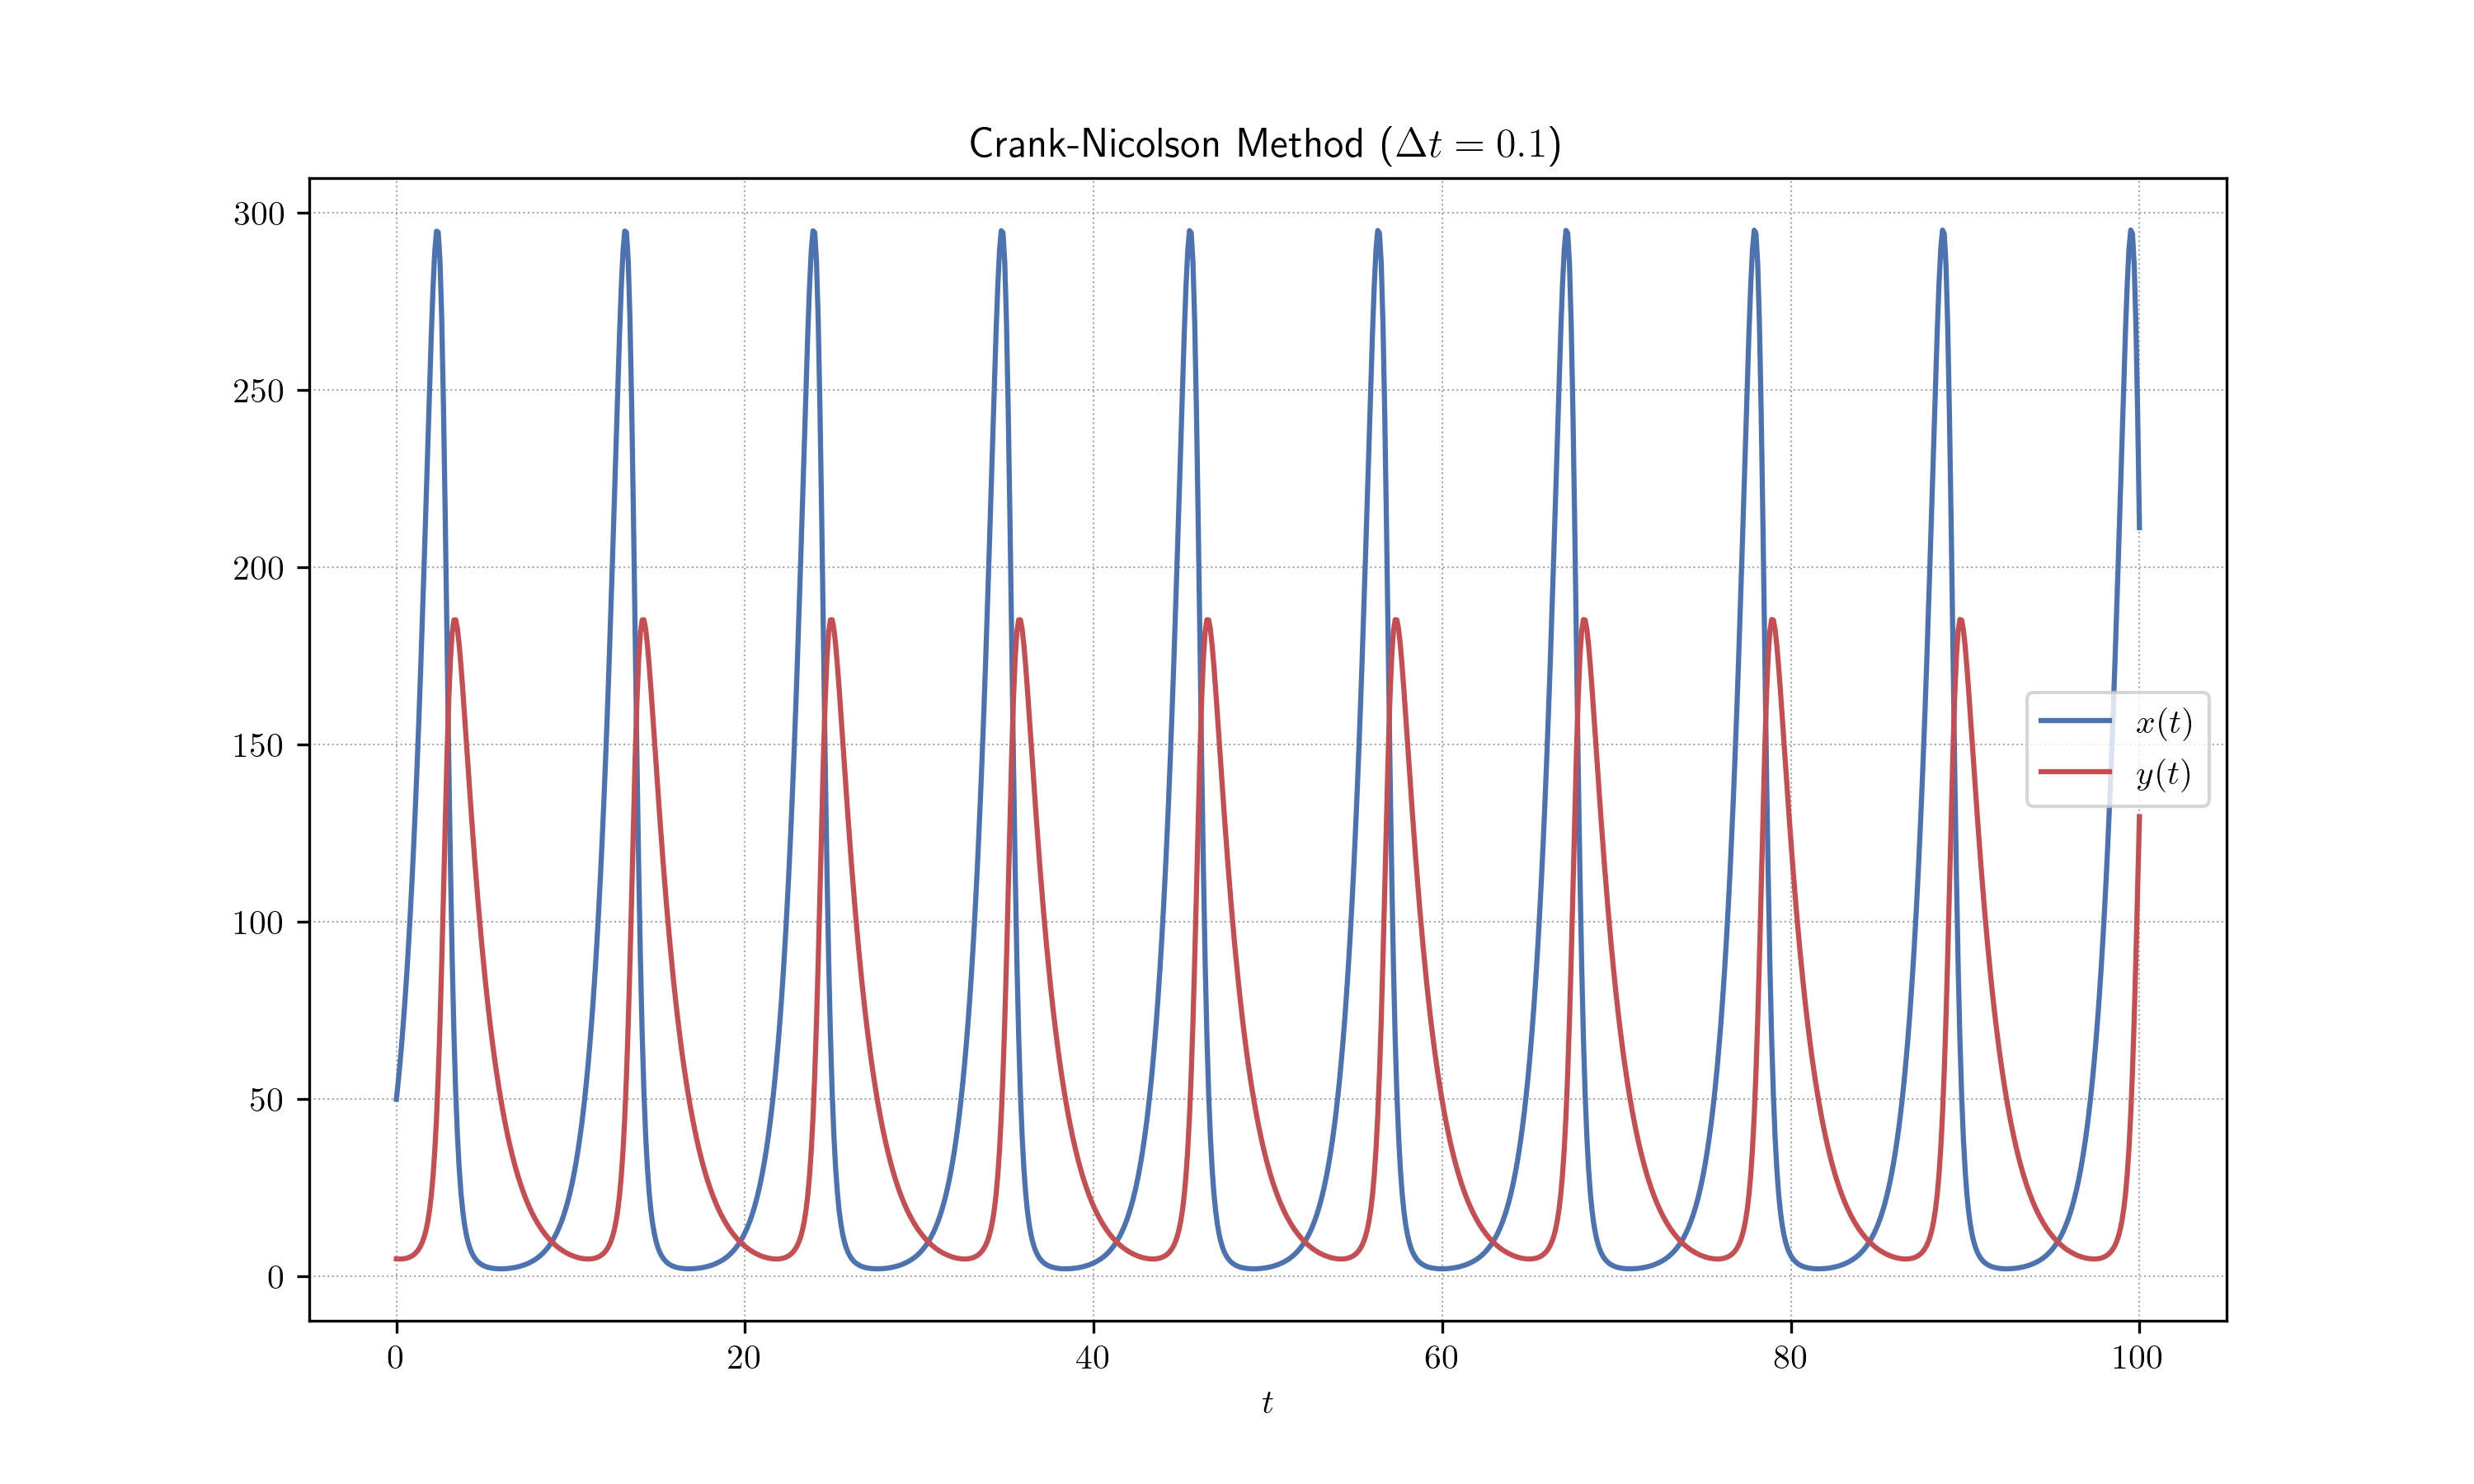
\includegraphics[width=0.75\textwidth]{../outputs/cn_0_1.png}
\end{center}

We note that the solution exhibits periodic behavior, which is consistent with the nature of the predator-prey systems. The populations of prey ($x$) and predators ($y$) oscillate over time, with the prey population peaking before the predator population follows suit. We can also observe the dependence of the predator population on the prey population by the nature of the fluctuations.\\

4. \textbf{Other Discussion Points.}
% \textbf{(a)} Lipshitz continuity of $f$.
% \newpage

\textbf{(a)} Plots of $x(t)$ and $y(t)$ over $[0,100]$ for $\Delta t \in \{0.025, 0.05, 0.1, 0.5, 0.8\}$.

In order of increasing time steps, the following plots are the results of our implementation:
\begin{center}
    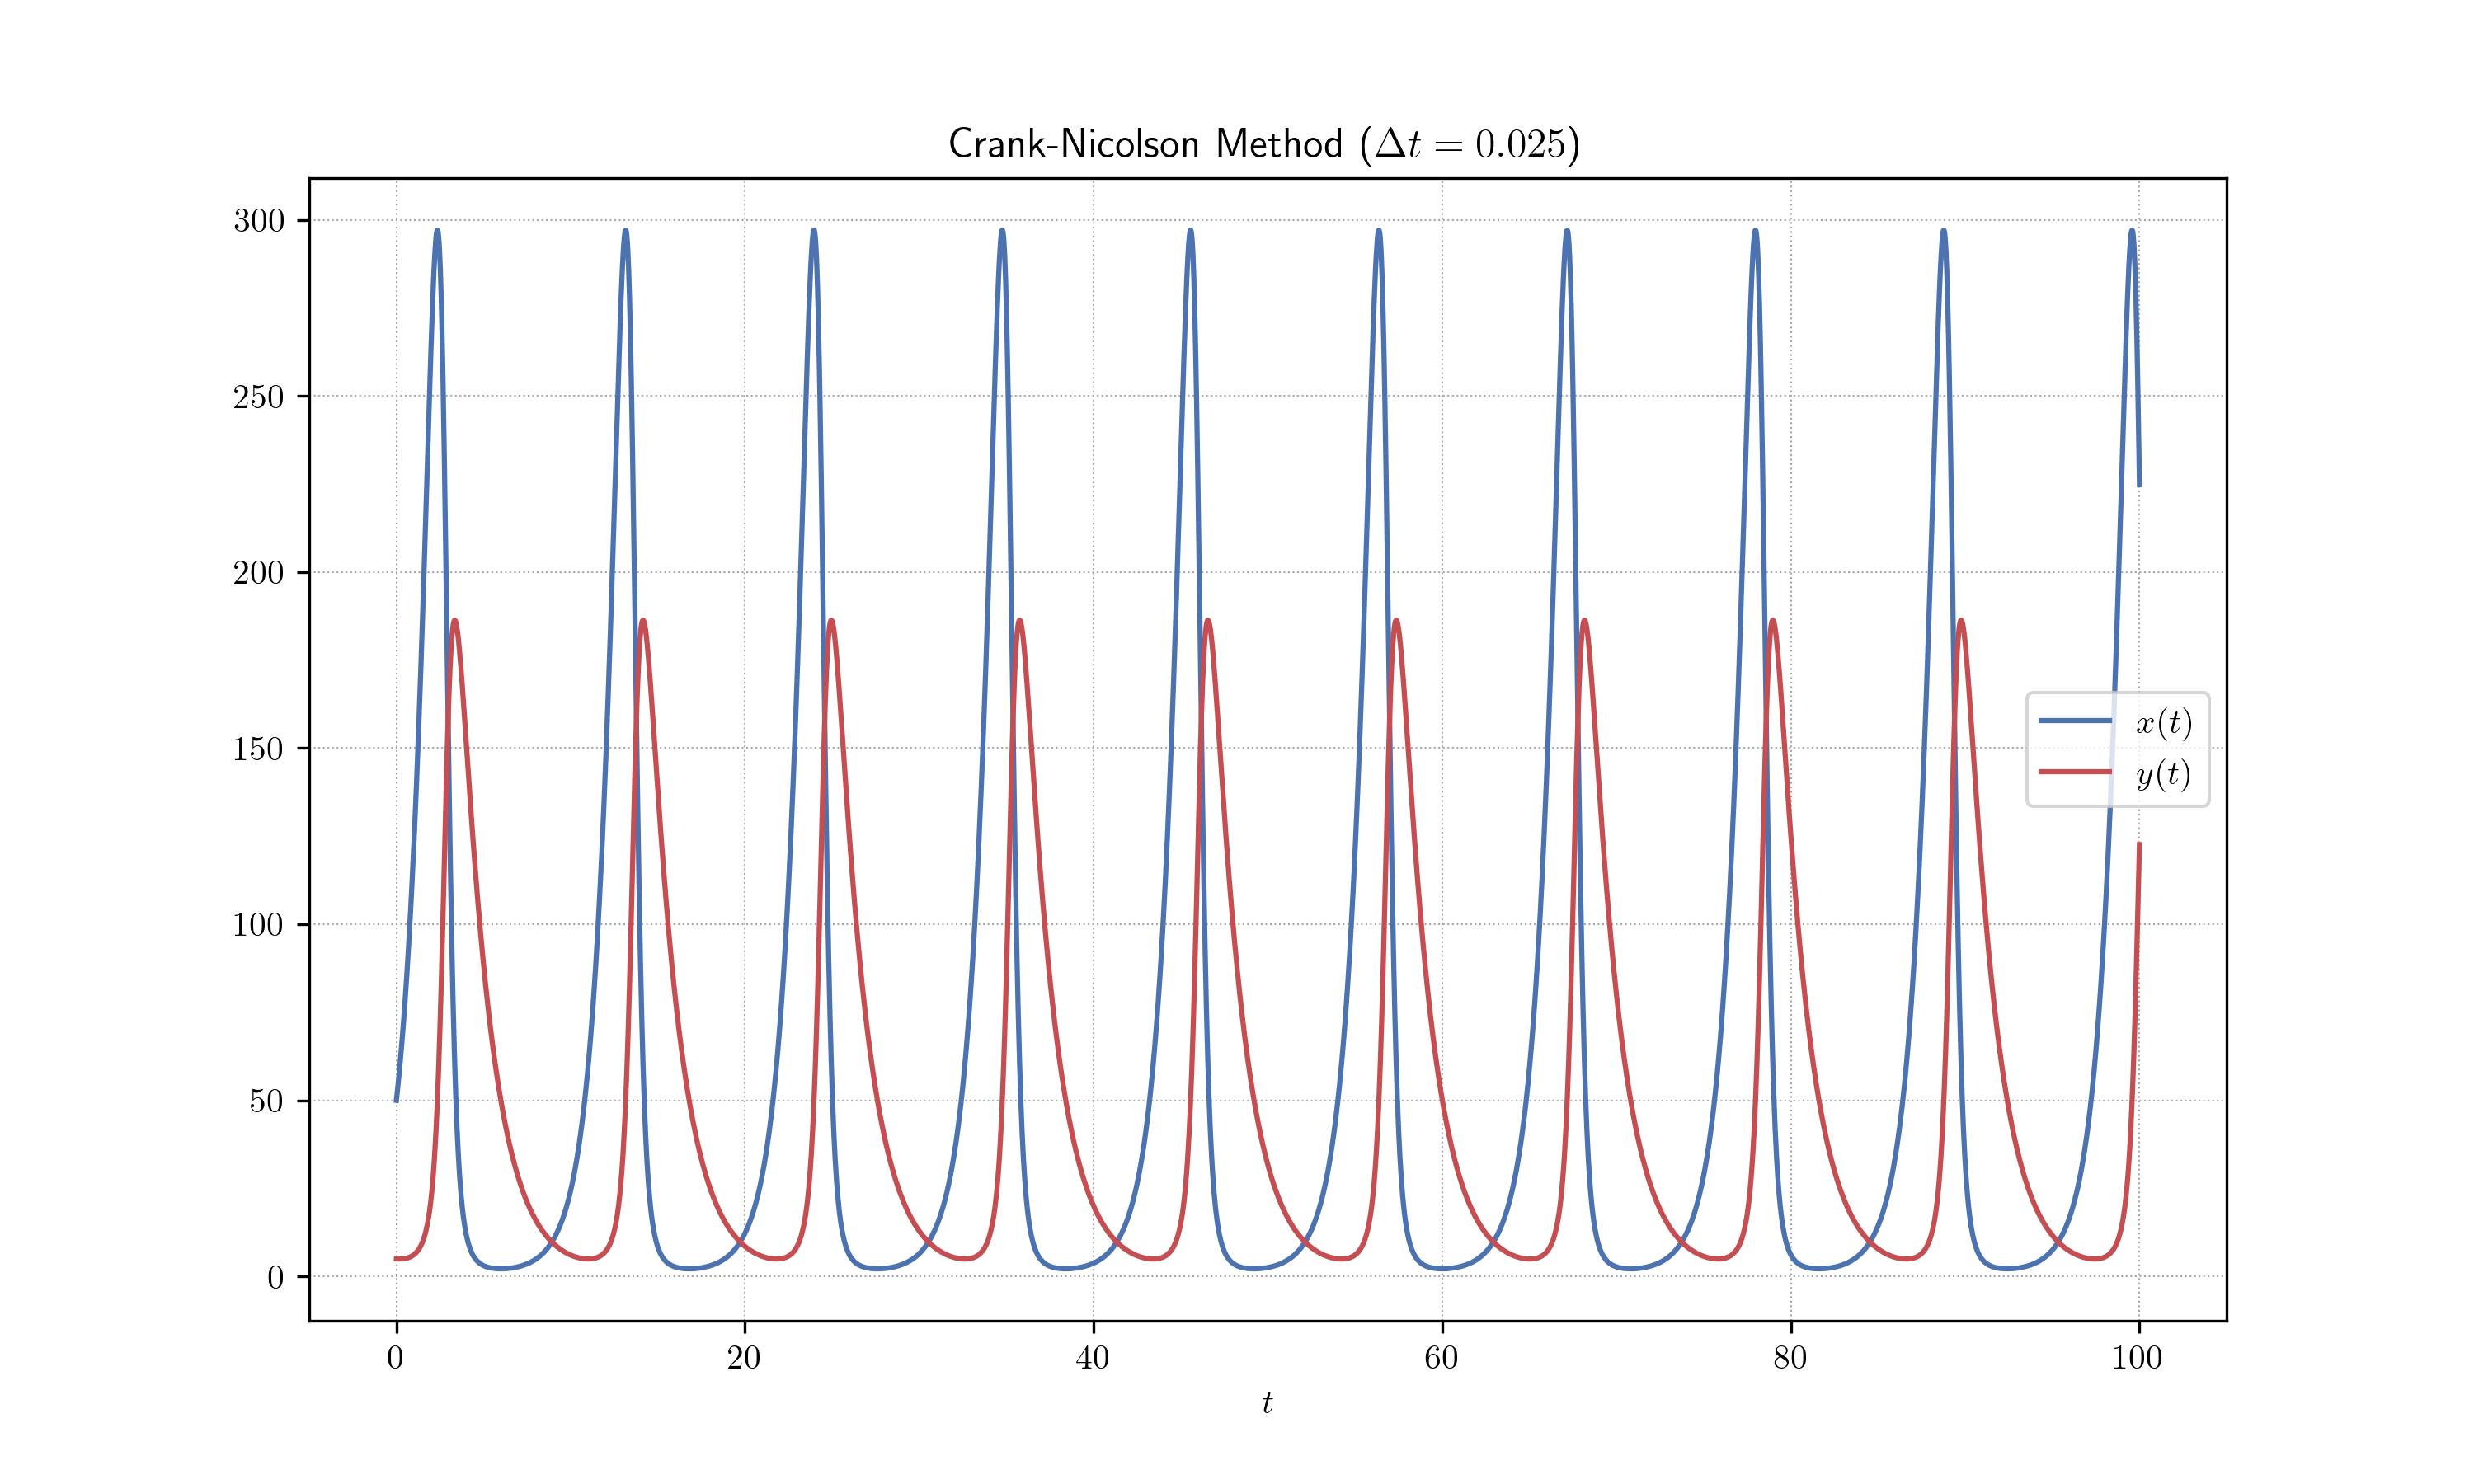
\includegraphics[width=0.75\textwidth]{../outputs/cn_0_025.png}
    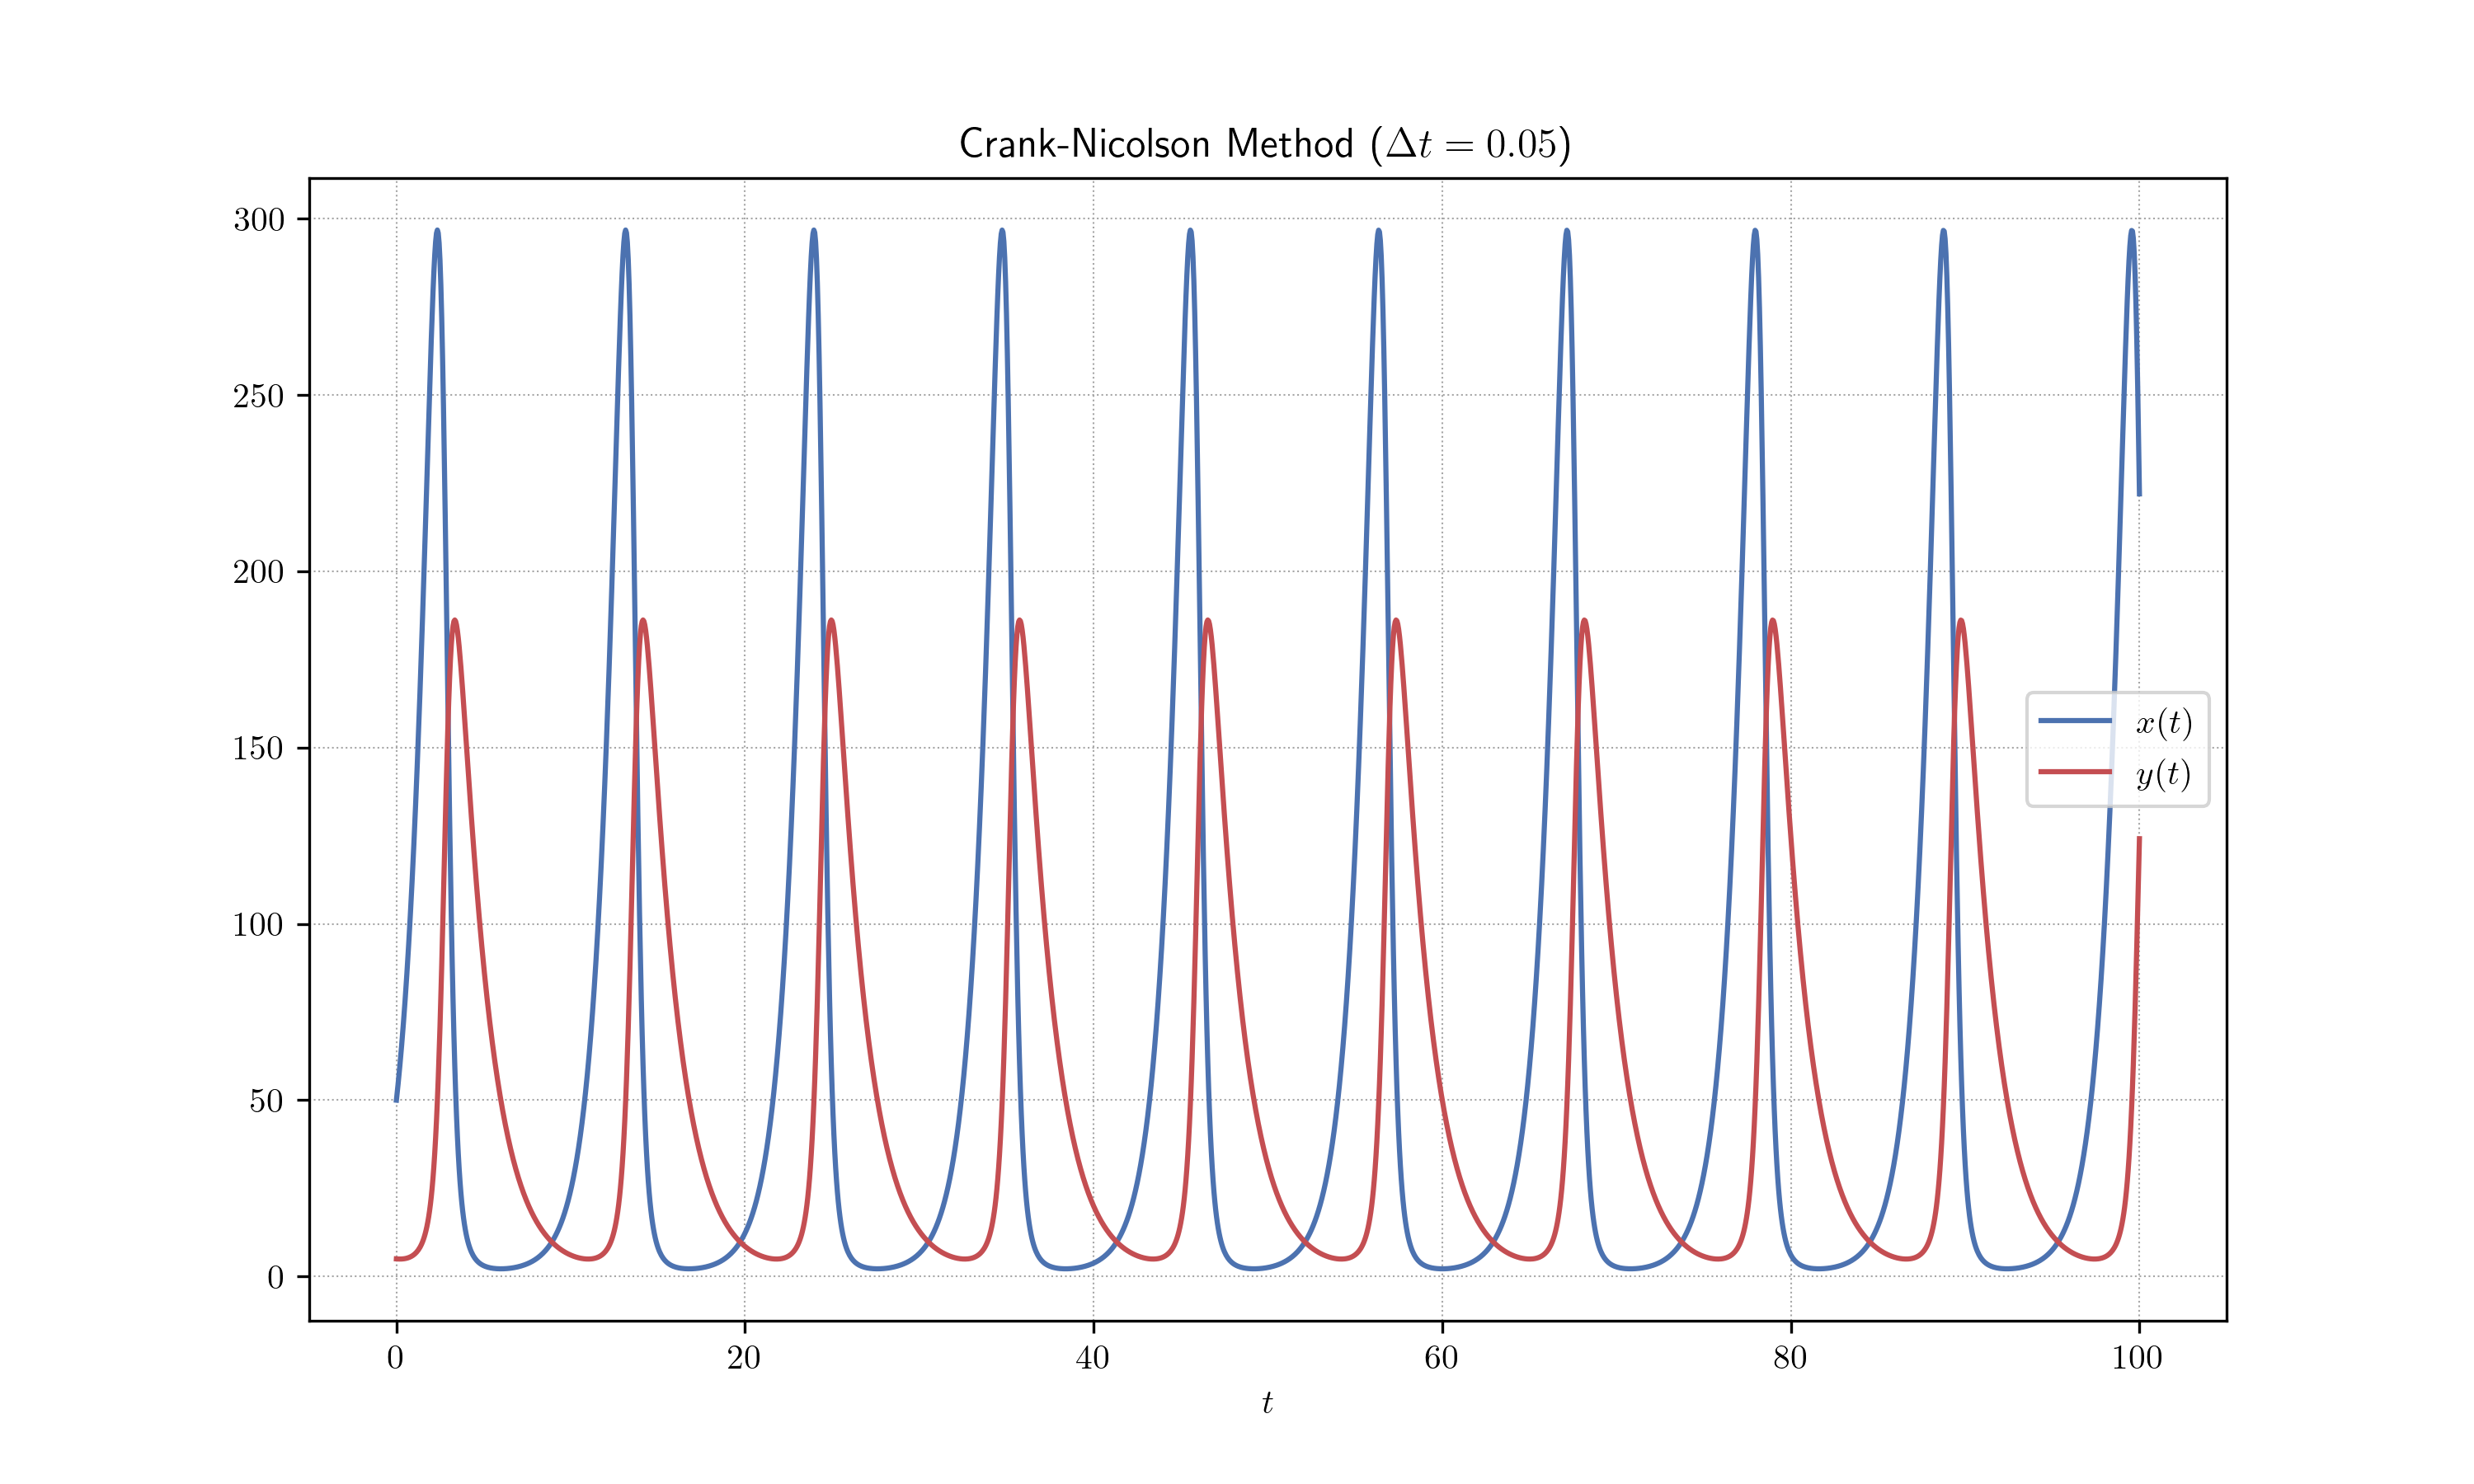
\includegraphics[width=0.75\textwidth]{../outputs/cn_0_05.png}
    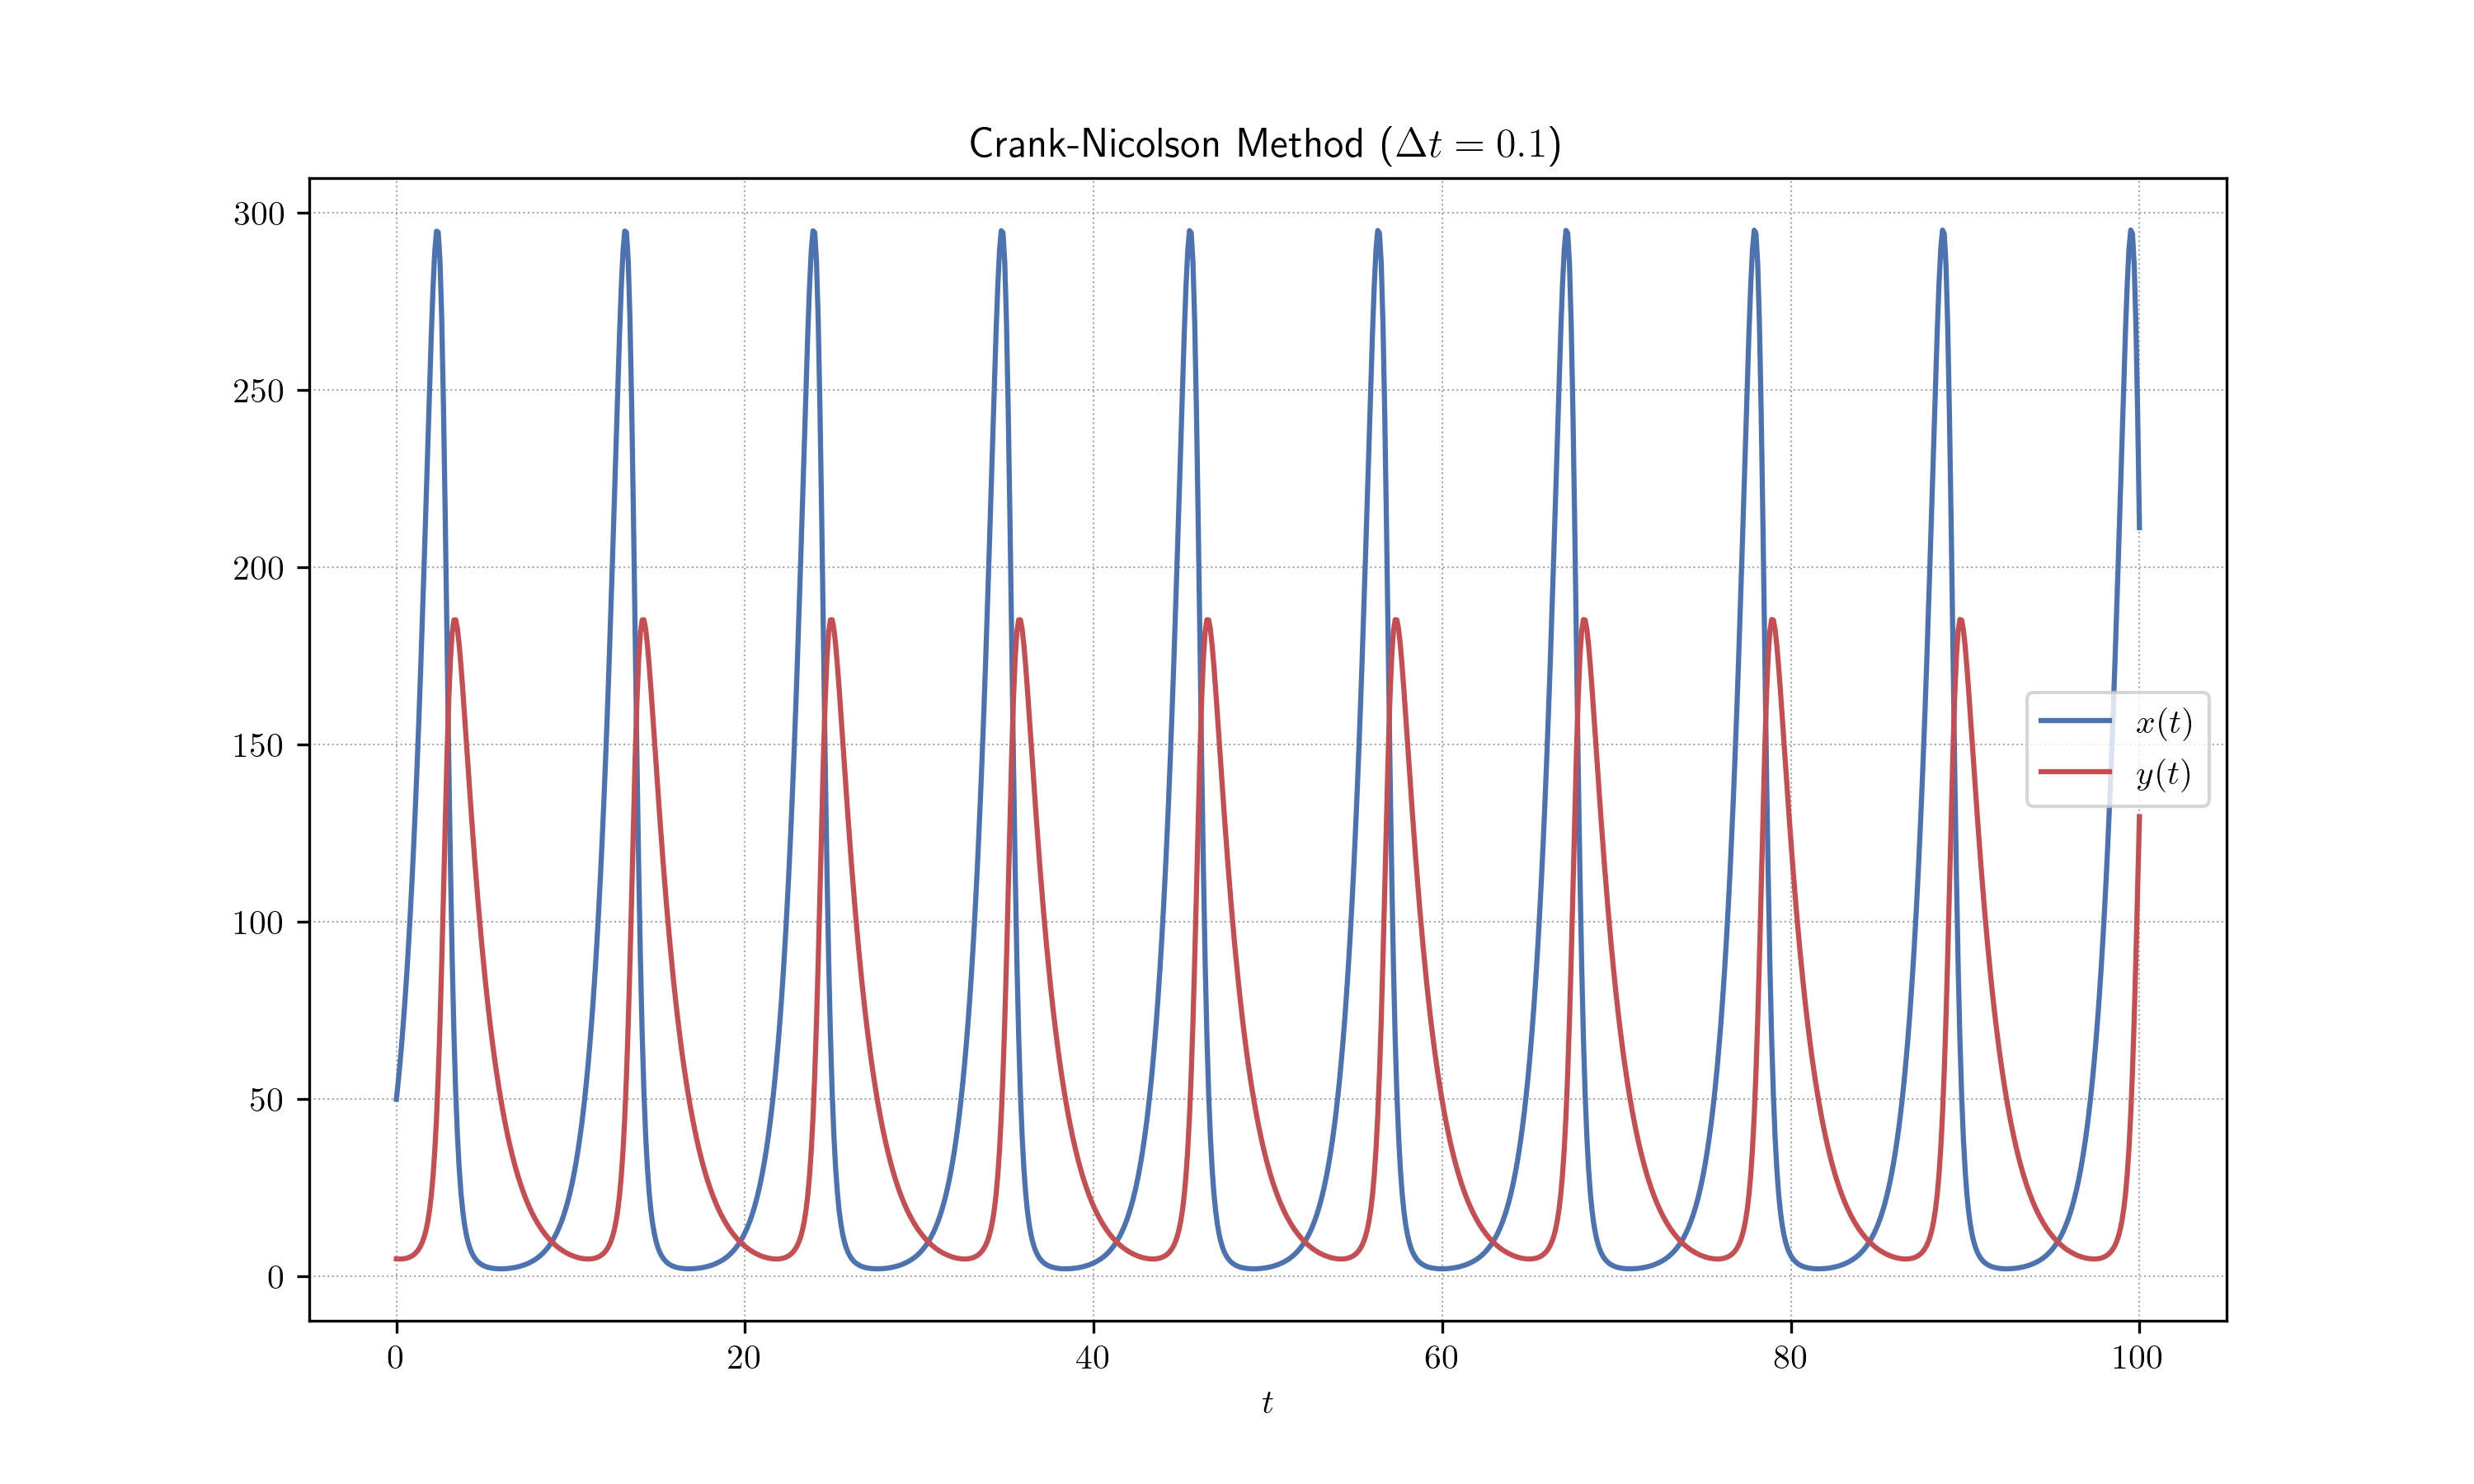
\includegraphics[width=0.75\textwidth]{../outputs/cn_0_1.png}
    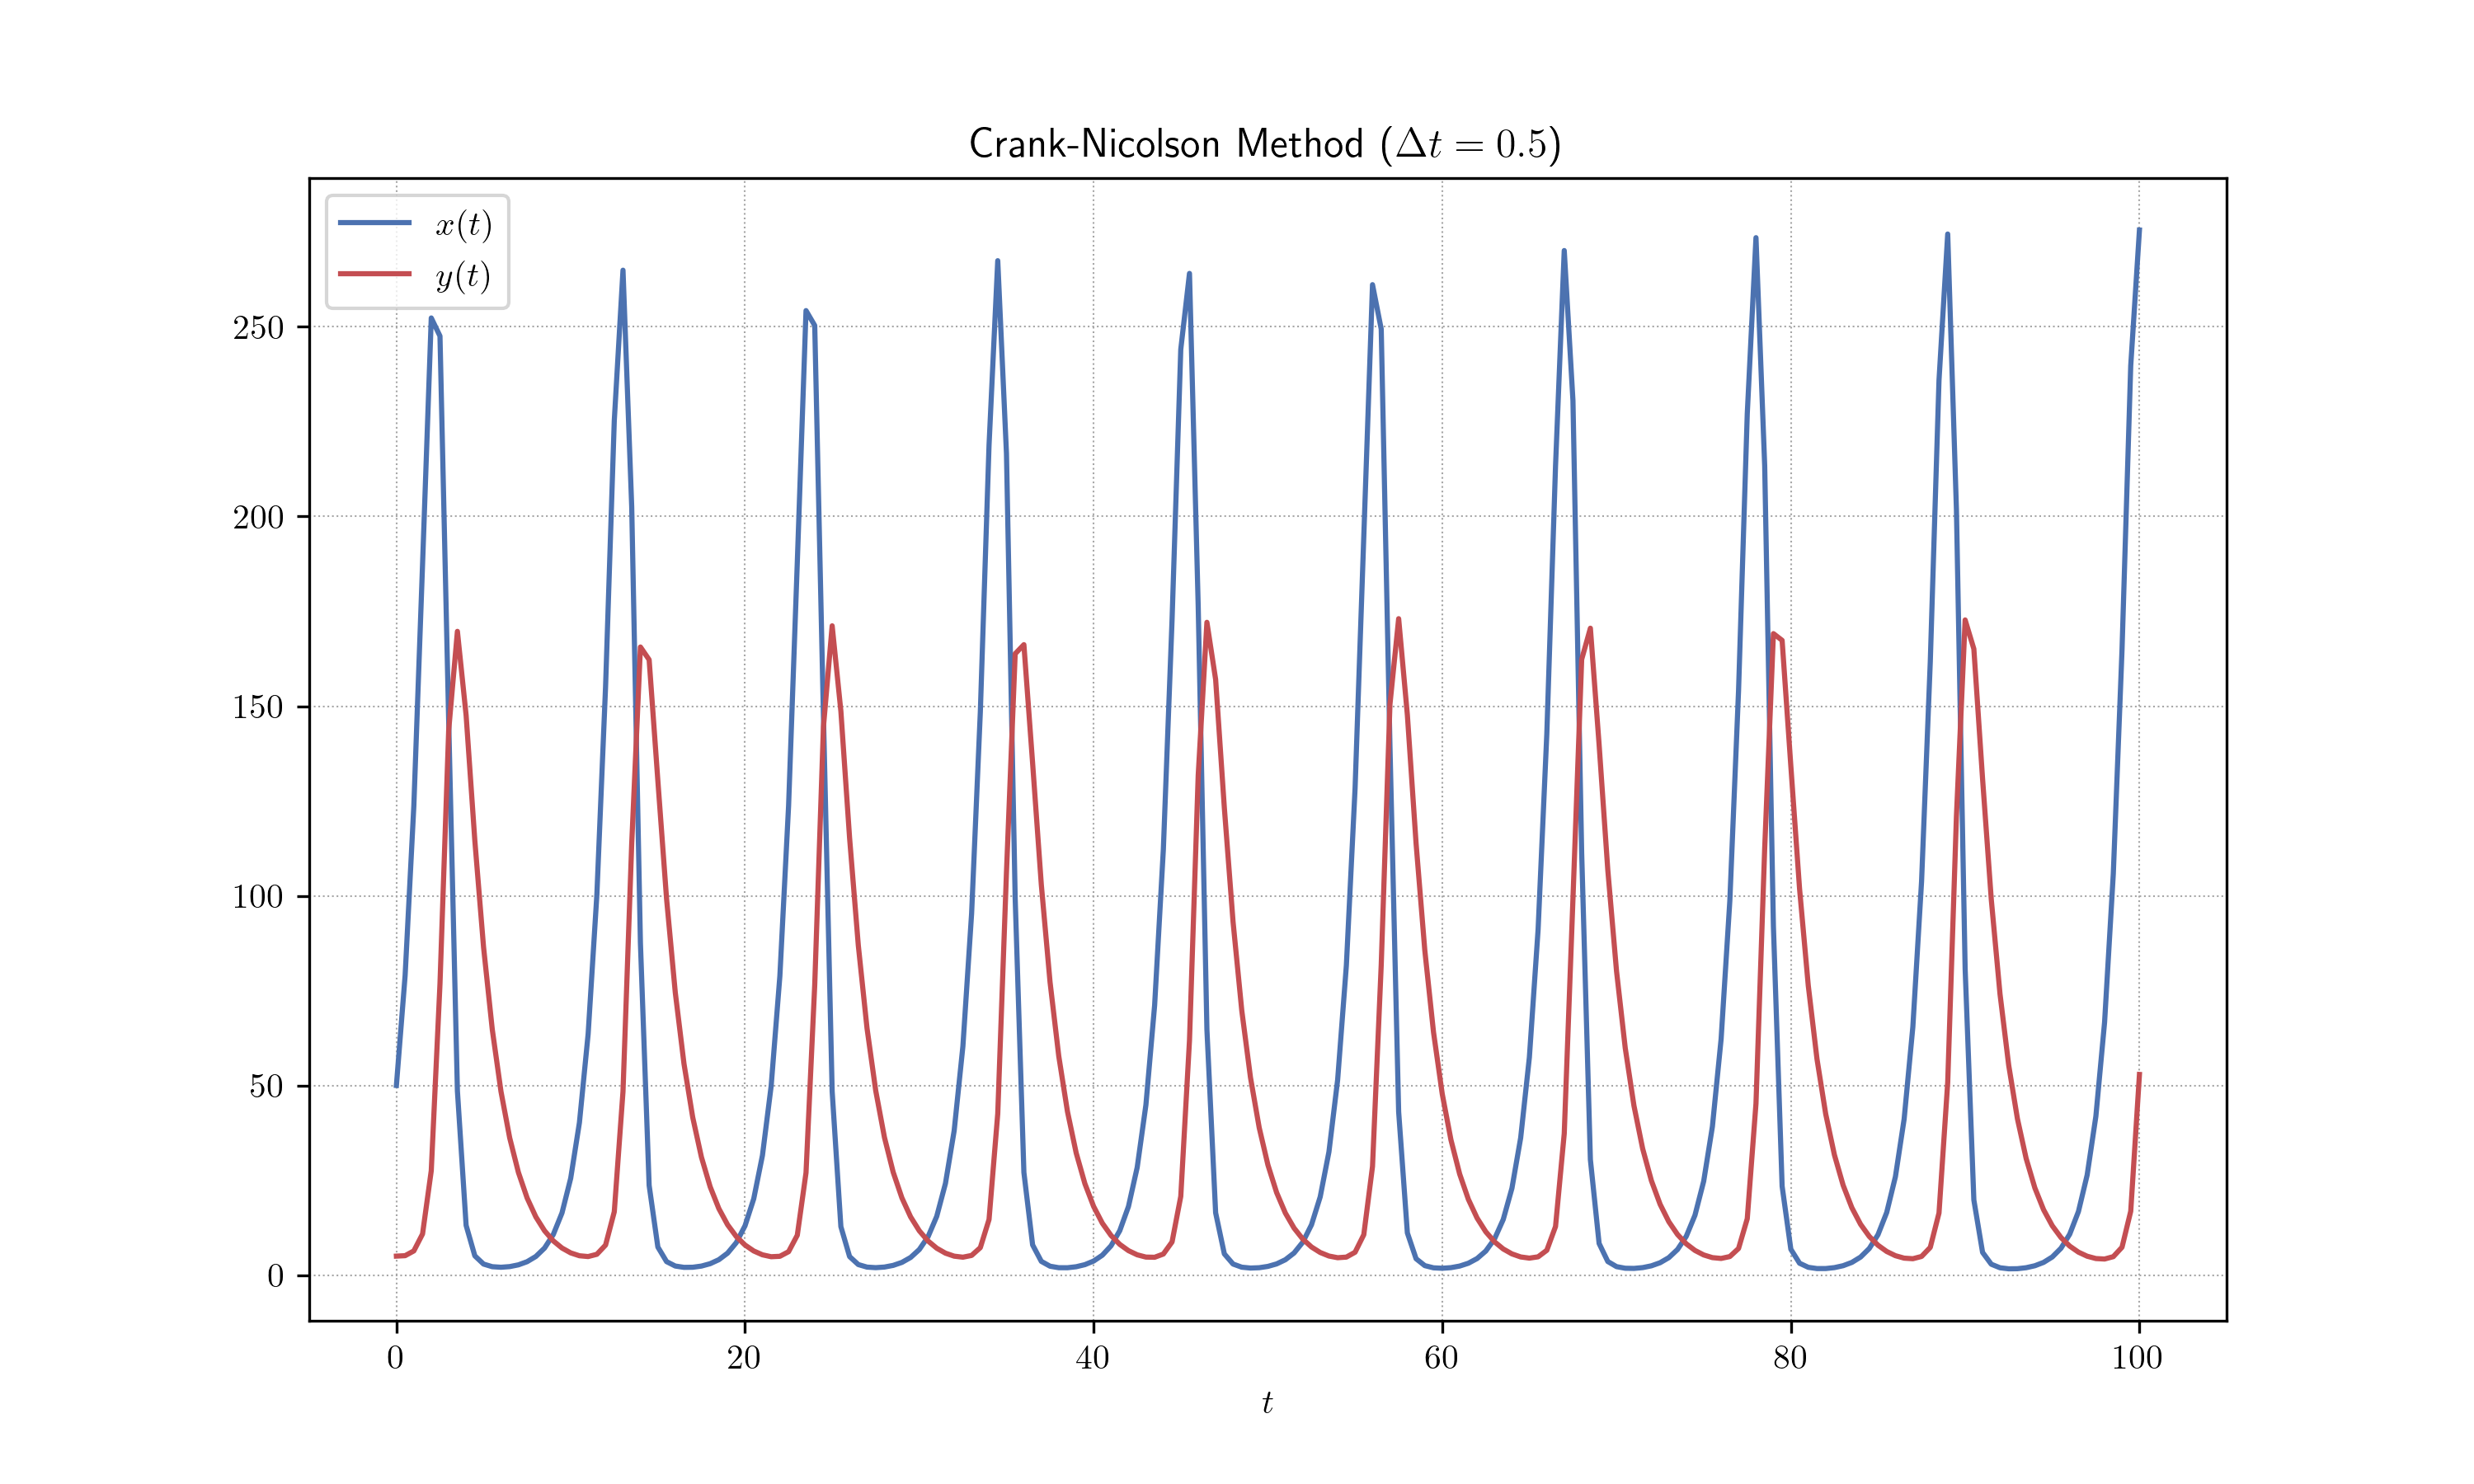
\includegraphics[width=0.75\textwidth]{../outputs/cn_0_5.png}
    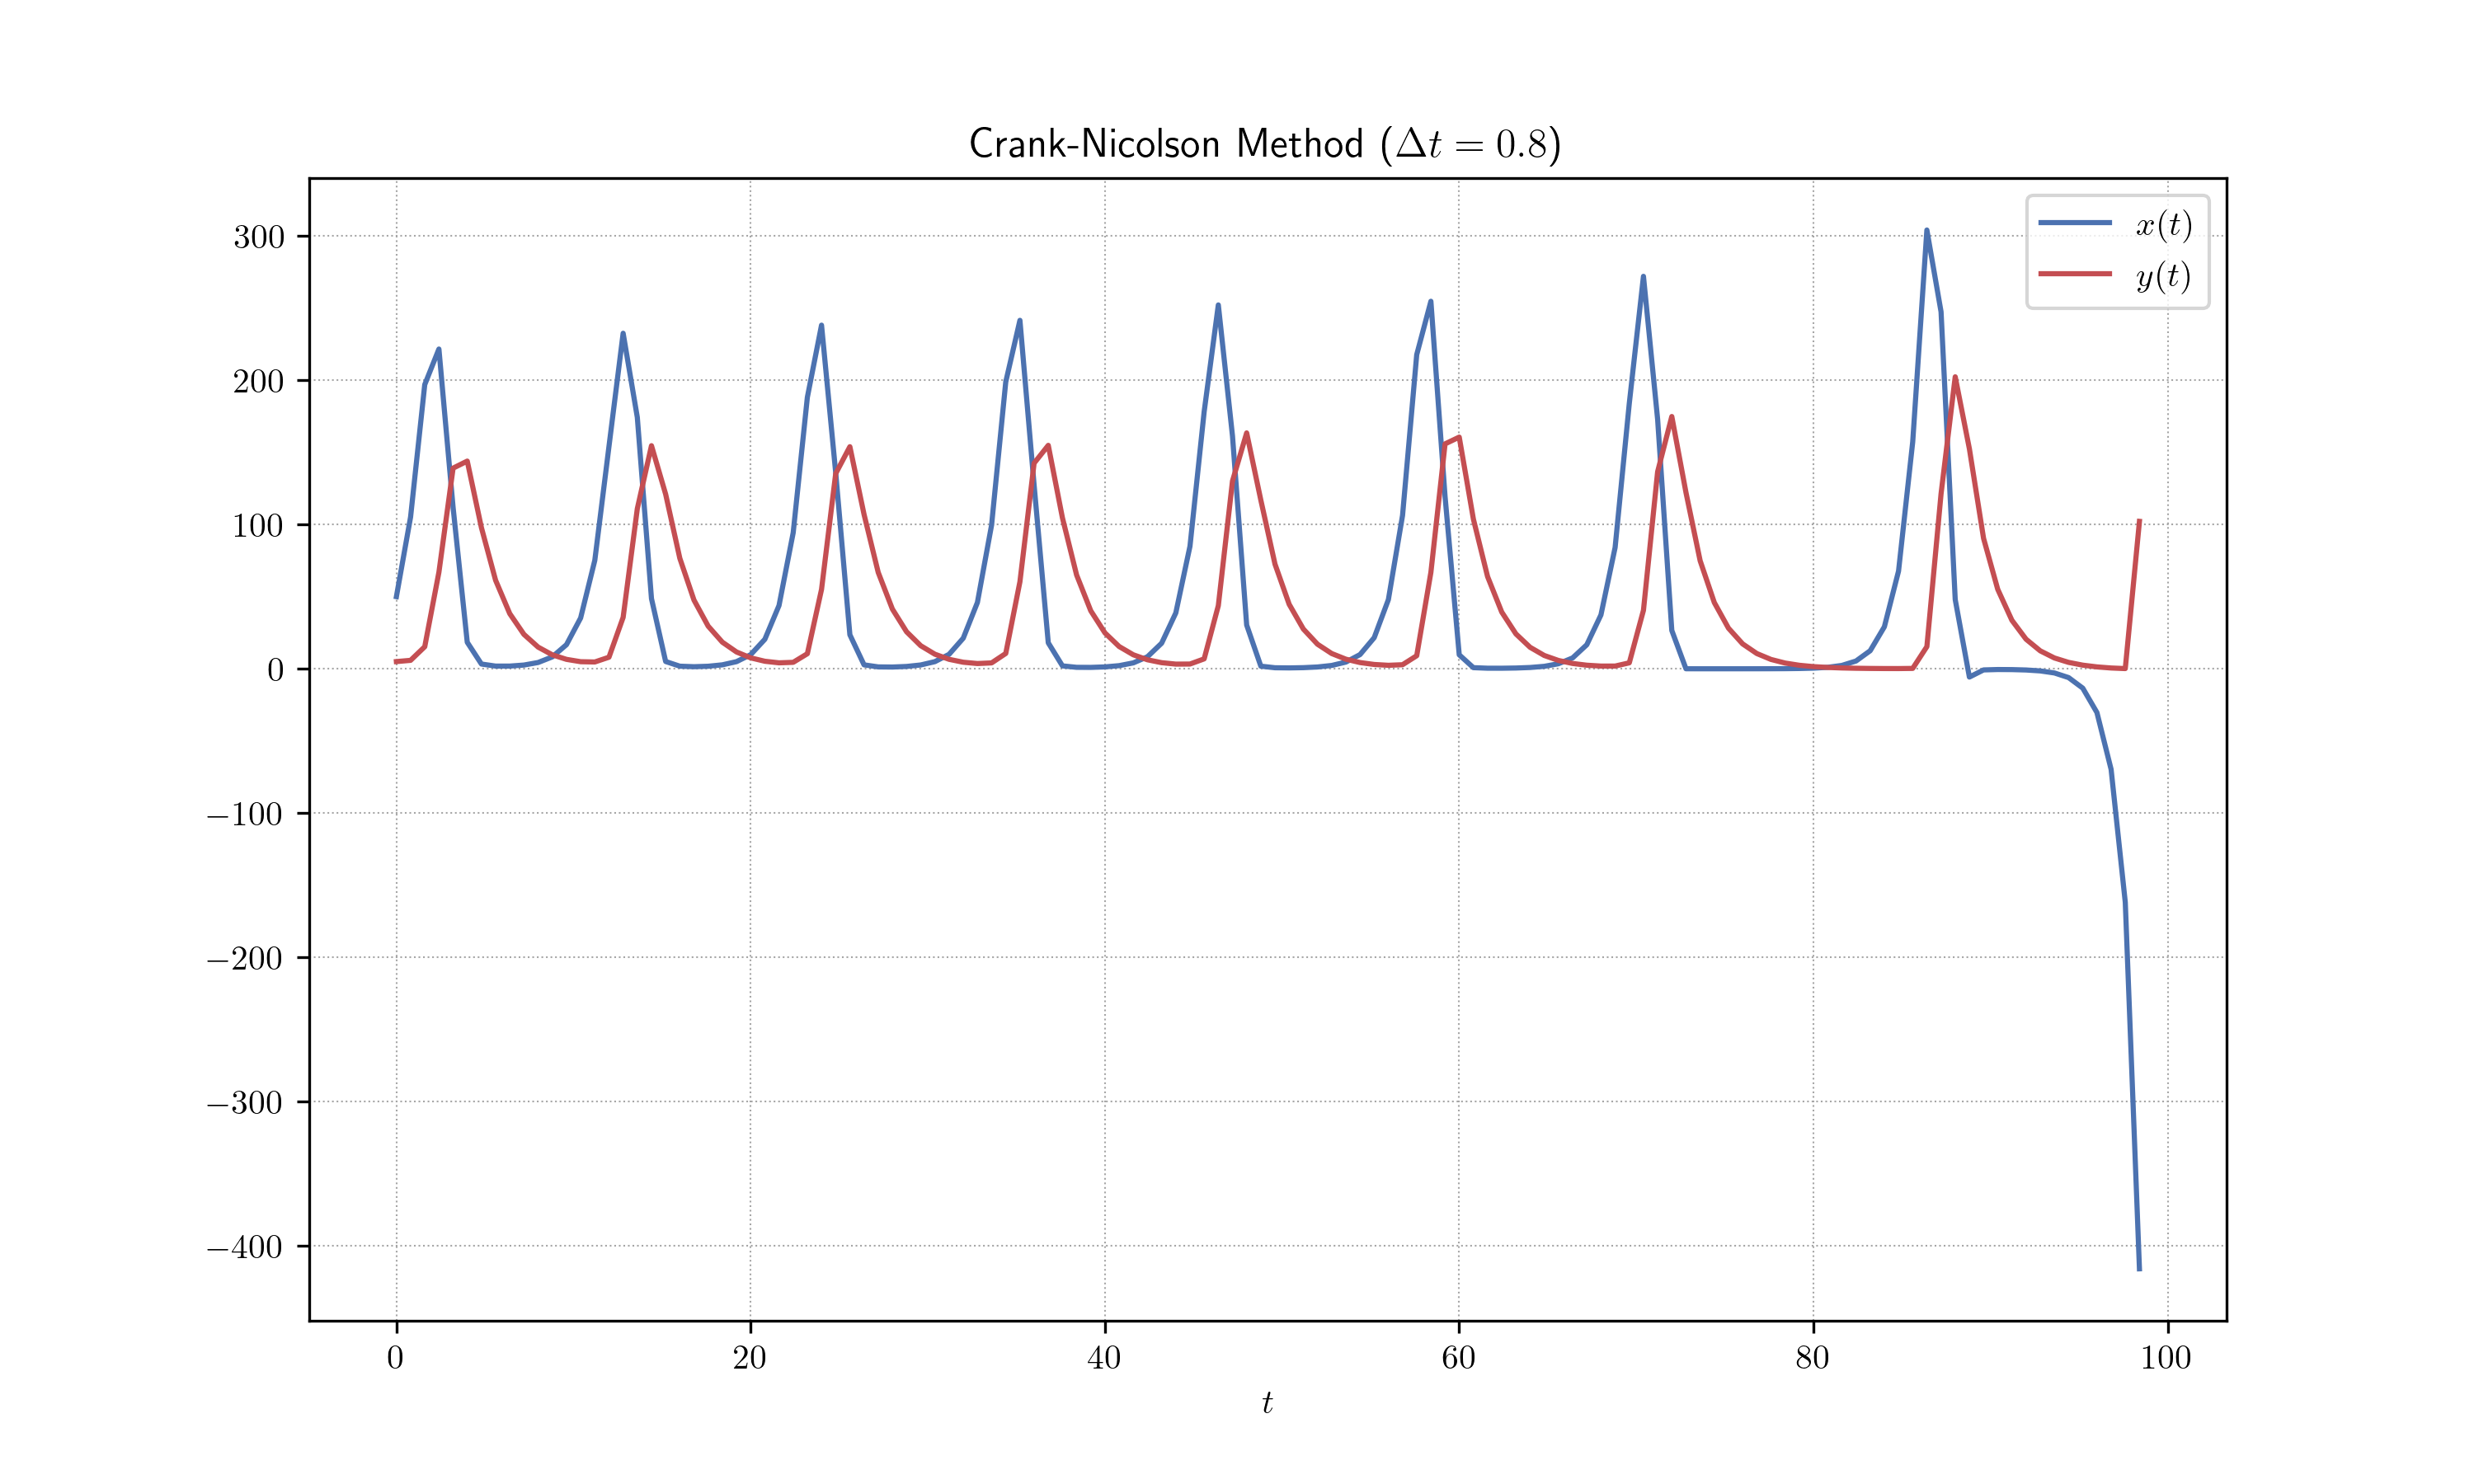
\includegraphics[width=0.75\textwidth]{../outputs/cn_0_8.png}
\end{center}

As a note, during code execution, overflow warnings were given for the largest timestep $\Delta t = 0.8$.

From the plots we observe that for $\Delta t \leq 0.1$, the solutions exhibit expected behavior. For $\Delta t = 0.5$, we see that the amplitudes of the solution starts to deviate from the expected periodic behavior. With long enough time, the solution may diverge from accumulated error. 

Then, for $\Delta t = 0.8$, the solution diverges significantly with $x(t)$ going negative, which is not physically meaningful in the context of population dynamics. 

Our observations suggest that for $\Delta t \geq 0.8$, the Picard operator associated with the Crank-Nicolson scheme is no longer a contraction for sufficiently large $t$. Which as a result, the convergence of the fixed point iteration is no longer guaranteed, leading to the divergence observed in the numerical solution.\\

\textbf{(b)} Phase plots of $y(t)$ vs $x(t)$ for $\Delta t \in \{0.025, 0.5\}$.

\begin{lstlisting}[language=Python, caption={Phase Plots Python}]
if __name__ == "__main__": # Was added to main from question 3
    h_values = [0.025, 0.5]
    file_name_labels = ['0_025', '0_5']
    for h, label in zip(h_values, file_name_labels):
        y_values = crank_nicolson_solver(h)
        plt.figure(figsize=(8, 8))
        plt.plot(y_values[:, 0], y_values[:, 1], label=rf"$\Delta t={h}$")
        plt.xlabel(r"$x(t)$")
        plt.ylabel(r"$y(t)$")
        plt.title(rf"Phase Plot ($\Delta t={h}$)")
        plt.legend()
        plt.savefig(f"./outputs/cn_phase_{label}.png", dpi=300)
        plt.cla()
\end{lstlisting}

The phase plots for $\Delta t = 0.025$ and $\Delta t = 0.5$ are as follows:
\begin{center}
    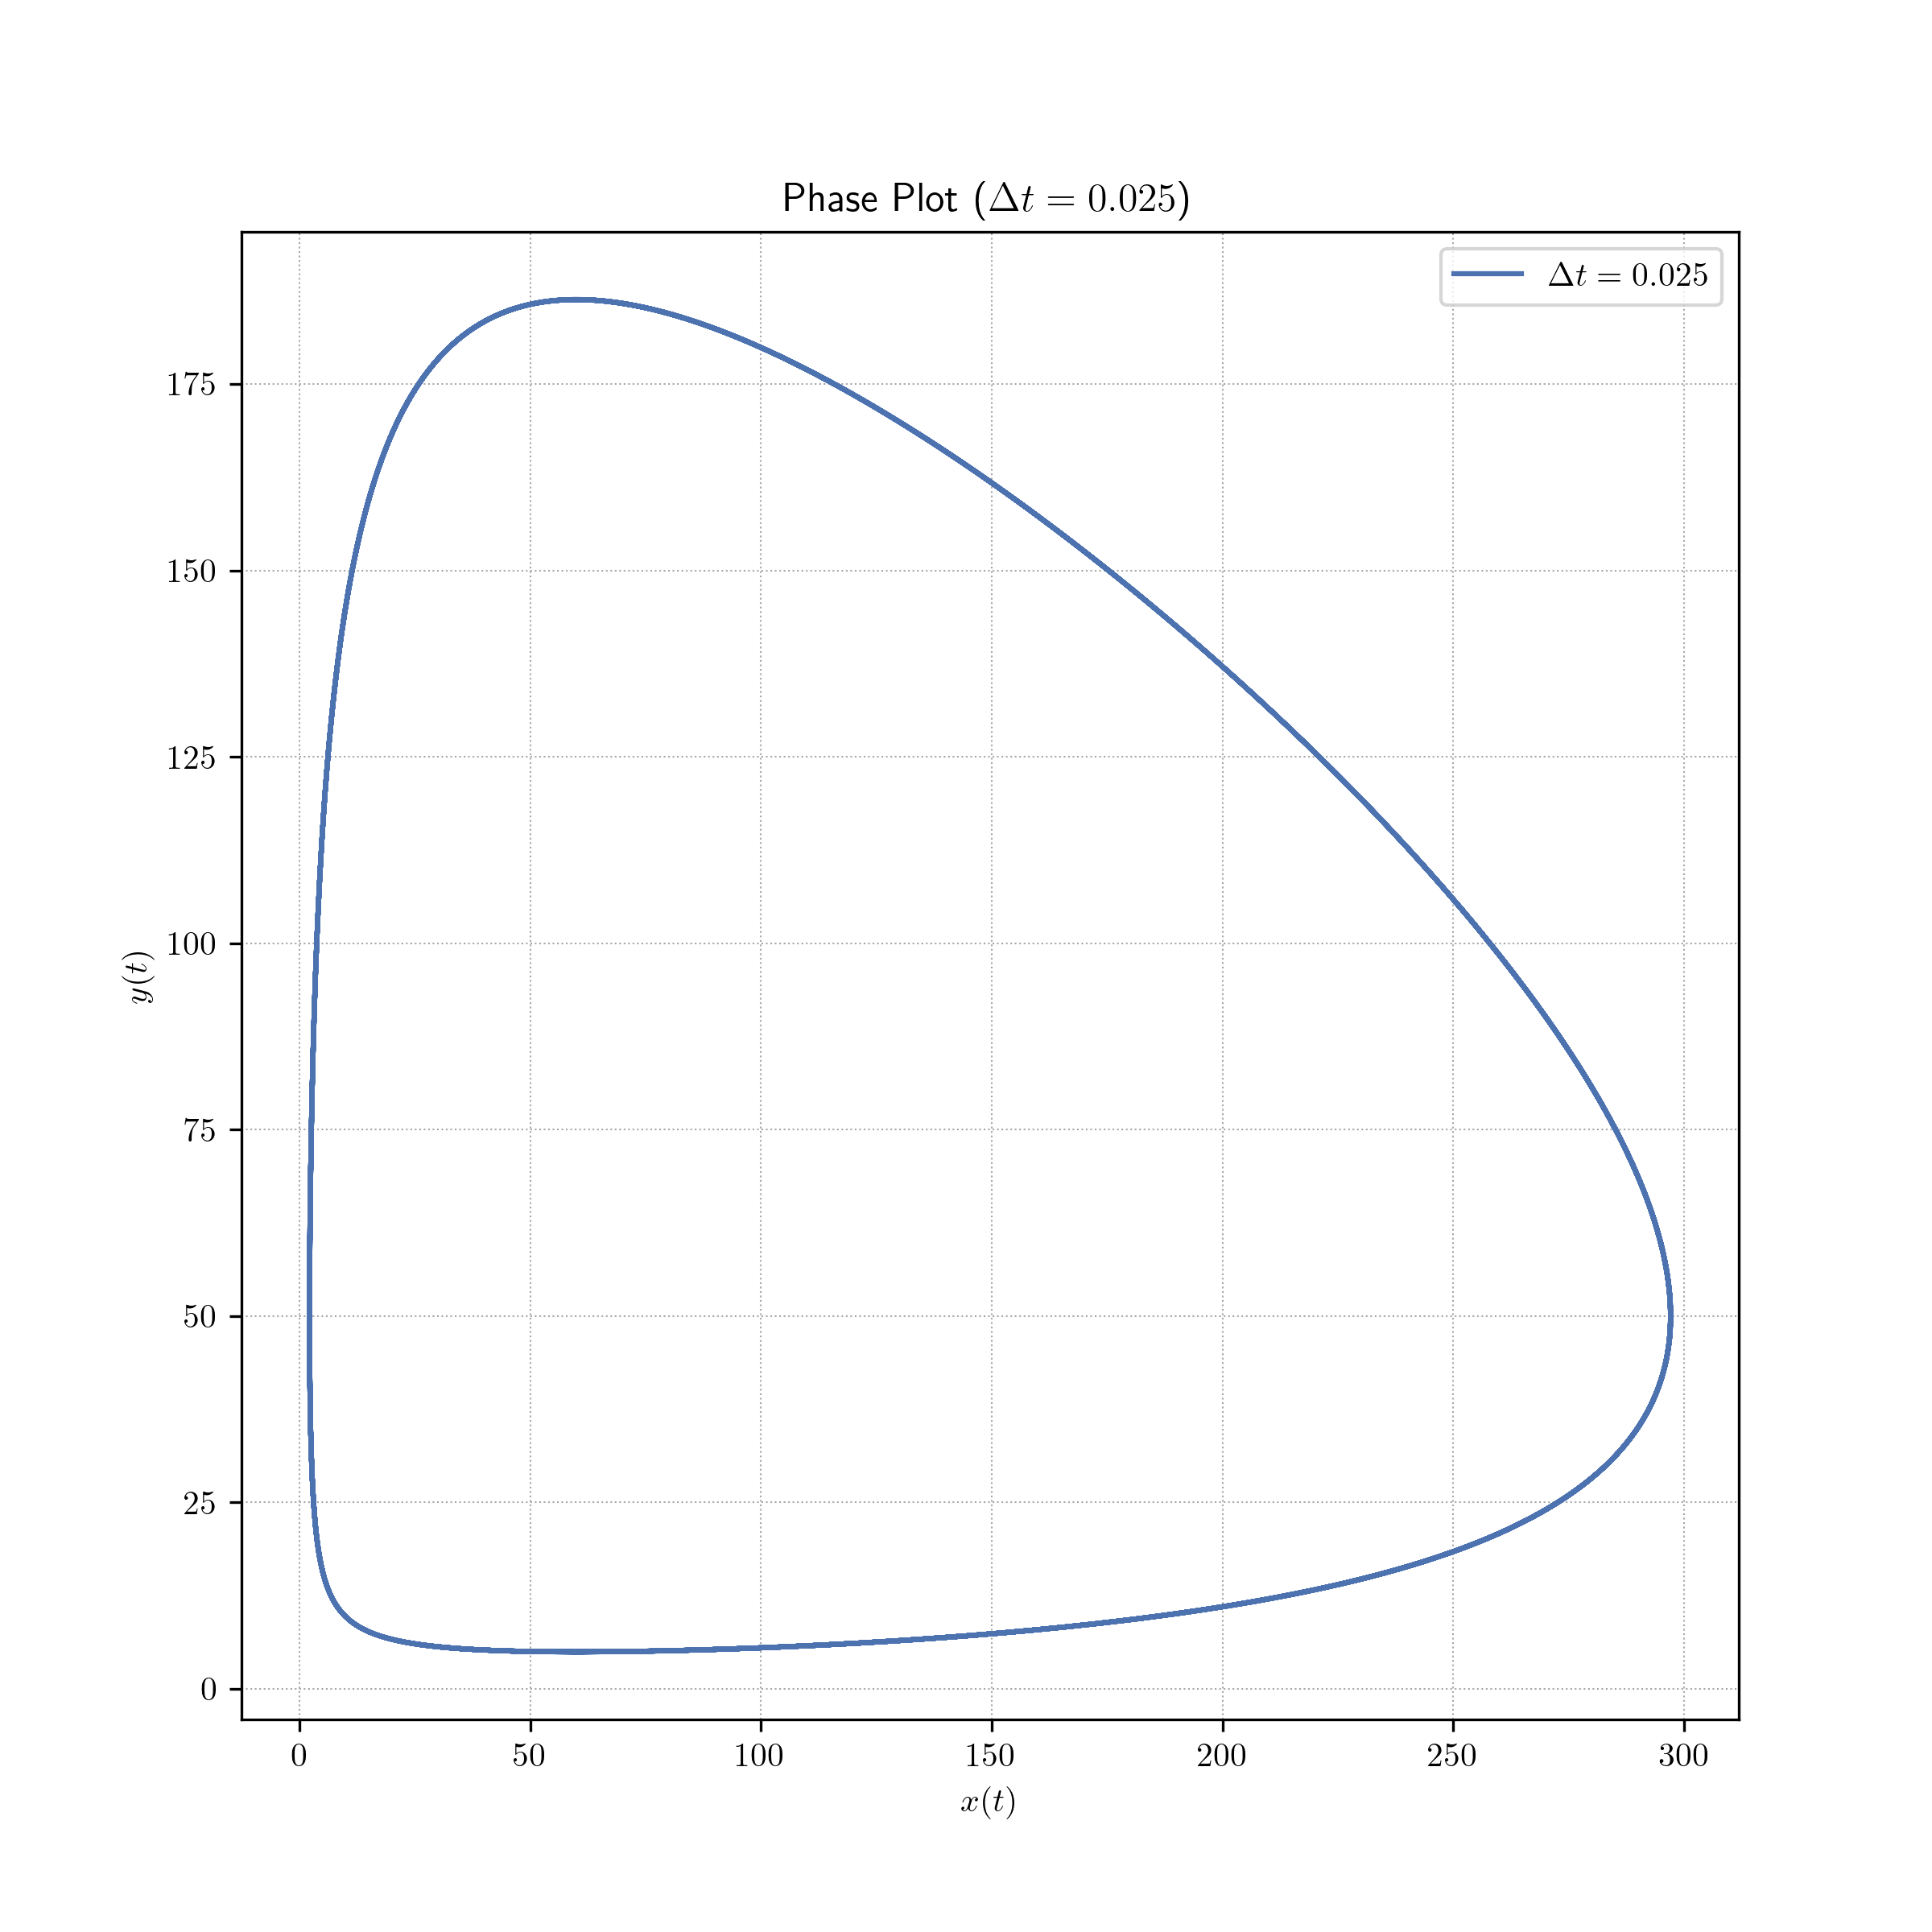
\includegraphics[width=0.65\textwidth]{../outputs/cn_phase_0_025.png}
    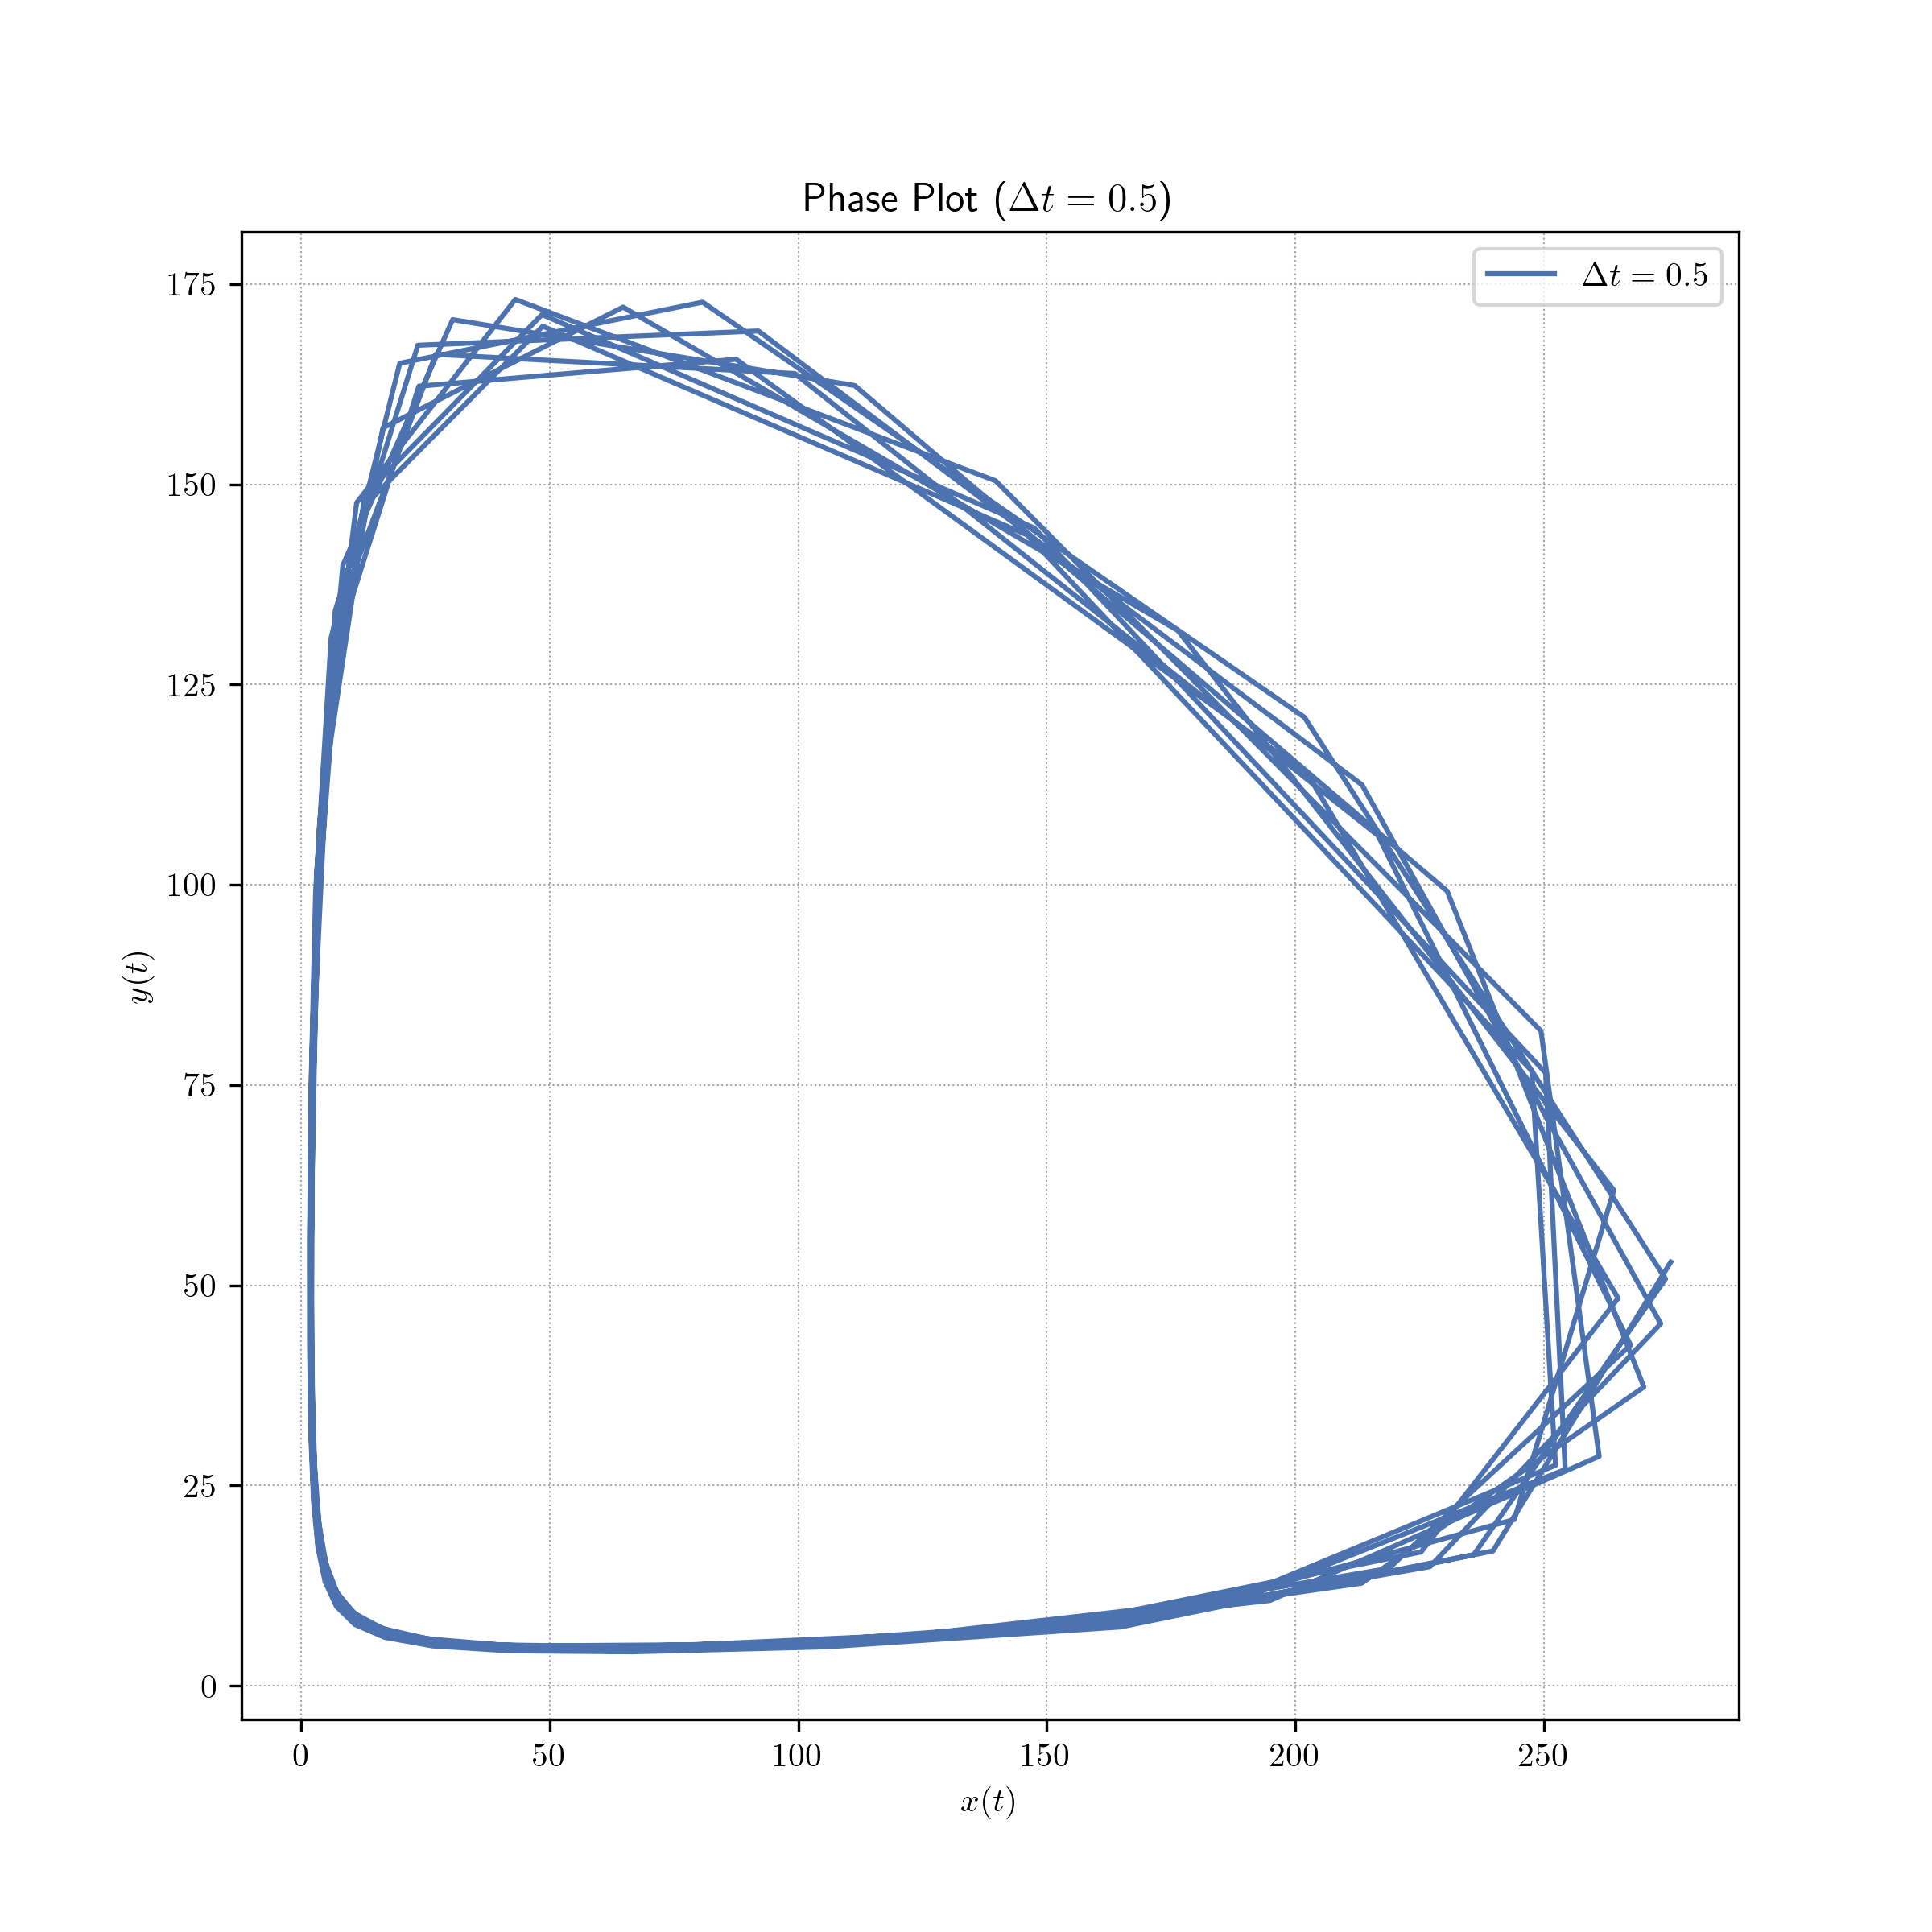
\includegraphics[width=0.65\textwidth]{../outputs/cn_phase_0_5.png}
\end{center}

We note that for $\Delta t = 0.025$, the phase plot exhibits a smooth, closed orbit, which is consistent with the expected periodic behavior. 

For $\Delta t = 0.5$, the phase plot maintains a closed orbit, but is noticeably more jagged and distorted. The discretization error is more pronounced, resulting in reduced resolution of the trajectories in the phase space. While the qualitative behavior of the system is still captured, the quantitative accuracy is compromised, which may lead to significant deviations over longer time intervals.

\end{document}